\section{Latches und FlipFlops}
\begin{center}
    \begin{minipage}[t]{0.45\linewidth}
        \paragraph{Kombinatorische Schaltung}
        Output hängt von Inputs und Verknüpfungen ab.
    \end{minipage}
    \hfill
    \begin{minipage}[t]{0.45\linewidth}
        \paragraph{Sequentielle Schaltung}
        Enthält Rückkopplungen, Outputs hängen von vorherigen Werten ab.
    \end{minipage}
\end{center}
\hrule
\begin{center}
    \begin{minipage}[t]{0.45\linewidth}
        \paragraph{Latch}
        \emph{(Takt)\underline{zustand}gesteurte} Schaltung $\rightarrow$ Änderungen am Eingang können während der \emph{ganzen aktiven Taktphase} den Output beeinflussen.
    \end{minipage}
    \hfill
    \begin{minipage}[t]{0.45\linewidth}
        \paragraph{FlipFlops}
        \emph{Takt\underline{flanken}gesteuerte} Schaltung $\rightarrow$ Input zum Zeitpunkt der Taktwechsels wird wirksam.
    \end{minipage}
\end{center}
\subsection{Latches}
Alle taktzustandgesteurte Schaltungen sind gegenüber \cemph[burntorange]{Störimpulsen} empfindlich, da bei $\text{T}=1$ jede Änderung übernommen wird.
\subsubsection{SR-Latch}
\begin{center}
    \begin{minipage}[c]{0.4\linewidth}
        \begin{circuit}
            \node[srLatch] (srlatch) {};
            \path[draw] (srlatch.pin 1) --++(180:0.4) node[fill = white] {\cirin{S}};
            \path[draw] (srlatch.pin 3) --++(180:0.4) node[fill = white] {\cirin{R}};
            \path[draw] (srlatch.pin 6) --++(0:0.4) node[fill = white] {\cirout{Q}};
            \path[draw] (srlatch.pin 4) --++(0:0.4) node[fill = white] {\ciroutn{Q}};
        \end{circuit}
    \end{minipage}
    \hfill
    \begin{minipage}[c]{0.55\linewidth}
        \begin{circuit}
            \node[nor port] (nor1) {};
            \node[nor port, below = 4mm of nor1] (nor2) {};

            \path[draw] (nor1.in 1) --++(180:0.6) node[fill = white] {\cirin{S}};
            \path[draw] (nor2.in 2) --++(180:0.6) node[fill = white] {\cirin{R}};

            \node[circ, right = 3mm of nor1.out] (nex1) {};
            \node[circ, right = 3mm of nor2.out] (nex2) {};

            \draw (nor1.out) -- (nex1) --++(270:0.3) -- ($(nor2.in 1) + (0, 0.25)$) -- (nor2.in 1);
            \draw (nor2.out) -- (nex2) --++(90:0.3) -- ($(nor1.in 2) - (0, 0.25)$) -- (nor1.in 2);

            \node[right = 12mm of nor1.out] (q) {\cirout{Q}};
            \node[right = 12mm of nor2.out] (notq) {\ciroutn{Q}};

            \draw (nex1) --++(0:0.2) -- ($(notq) - (0.4, 0)$) -- (notq);
            \draw (nex2) --++(0:0.2) -- ($(q) - (0.4, 0)$) -- (q);
        \end{circuit}
    \end{minipage}
\end{center}
\begin{flushleft}
    \begin{tabular}{l l c l}
        \textbf{S} & Set & $\rightarrow$ & setzt $Q$ auf $1$\\
        \textbf{R} & Reset & $\rightarrow$ & setzt $Q$ auf $0$\\
    \end{tabular}
\end{flushleft}
\begin{equation*}
    Q_{n + 1} = S \lor \left(Q_n \land \overline{R}\right)
\end{equation*}
\begin{center}
    \begin{tabular}{c|c c|c l}
        Fall & \textbf{S} & \textbf{R} & $Q_{n + 1}$ & \\
        \cline{1-4}
        1 & $0$ & $0$ & $Q_n$ & speichern\\        
        2 & $0$ & $1$ & $0$ & zurücksetzten\\        
        3 & $1$ & $0$ & $1$ & setzen\\        
        4 & $1$ & $1$ & - & unzulässig\\        
    \end{tabular}
\end{center}
\subsubsection{SRT-Latch}
\begin{center}
    \begin{minipage}[c]{0.4\linewidth}
        \begin{circuit}
            \node[srtLatch] (srtlatch) {};
            \path[draw] (srtlatch.pin 1) --++(180:0.4) node[fill = white] {\cirin{S}};
            \path[draw] (srtlatch.pin 2) --++(180:0.4) node[fill = white] {\cirin{T}};
            \path[draw] (srtlatch.pin 3) --++(180:0.4) node[fill = white] {\cirin{R}};
            \path[draw] (srtlatch.pin 6) --++(0:0.4) node[fill = white] {\cirout{Q}};
            \path[draw] (srtlatch.pin 4) --++(0:0.4) node[fill = white] {\ciroutn{Q}};
        \end{circuit}
    \end{minipage}
    \hfill
    \begin{minipage}[c]{0.55\linewidth}
        \begin{circuit}
            \node[and port] (and1) at (0, 0.5) {};
            \node[and port] (and2) at (0, -0.5) {};
            \node[srLatch] (srlatch) at (1.1,0) {};

            \node[left = 4mm of and1.in 1] (sin) {\cirin{S}};
            \node[left = 4mm of and2.in 2] (rin) {\cirin{S}};
            \node[] at ($(sin)!0.5!(rin)$) (tin) {\cirin{T}};
            \node[right = 3mm of srlatch.pin 6] (q) {\cirout{Q}};
            \node[right = 3mm of srlatch.pin 4] (notq) {\ciroutn{Q}};

            \draw[] (sin) -- (and1.in 1); 
            \draw[] (rin) -- (and2.in 2); 
            \draw[] (tin) --++(0:0.5) |- (and1.in 2);
            \draw[] (tin) --++(0:0.5) |- (and2.in 1);

            \draw(srlatch.pin 6) -- (q);
            \draw(srlatch.pin 4) -- (notq);

            \draw[] (and1.out) --++(0:0.2) node[label={[label distance = -2mm, font = \small]20:$\text{S}_{\text{int}}$}]{} |- (srlatch.pin 1);
            \draw[] (and2.out) --++(0:0.2) node[label={[label distance = -2mm, font = \small]340:$\text{R}_{\text{int}}$}]{} |- (srlatch.pin 3);
        \end{circuit}
    \end{minipage}
\end{center}
\begin{flushleft}
    \begin{tabular}{c c c c c l}
        T & & $\text{S}_{\text{int}}$ & $\text{R}_{\text{int}}$ & &\\
        $0$ & $\rightarrow$ & $0$ & $0$ & $\rightarrow$ & Datenspeicherung\\
        $1$ & $\rightarrow$ & S & R & $\rightarrow$ & Normales SR-Latch\\
    \end{tabular}
\end{flushleft}
Änderungen werden nur übernommen, wenn T/CLK aktiv ist.

\subsubsection{D-Latch}
\begin{center}
    \begin{minipage}[c]{0.4\linewidth}
        \begin{circuit}
            \node[dLatch] (dlatch) {};
            \path[draw] (dlatch.pin 1) --++(180:0.4) node[fill = white] {\cirin{D}};
            \path[draw] (dlatch.pin 2) --++(180:0.4) node[fill = white] {\cirin{T}};
            \path[draw] (dlatch.pin 6) --++(0:0.4) node[fill = white] {\cirout{Q}};
            \path[draw] (dlatch.pin 4) --++(0:0.4) node[fill = white] {\ciroutn{Q}};
        \end{circuit}
    \end{minipage}
    \hfill
    \begin{minipage}[c]{0.55\linewidth}
        \begin{circuit}
            \node[srtLatch] (srtlatch) {};

            \node[left = 14mm of srtlatch.pin 1] (din) {\cirin{D}};
            \node[left = 14mm of srtlatch.pin 2] (tin) {\cirin{T}};
            \node[right = 2mm of srtlatch.pin 6] (q) {\cirout{Q}};
            \node[right = 2mm of srtlatch.pin 4] (notq) {\ciroutn{Q}};

            \node[not port, left = 2mm of srtlatch.pin 3] (not) {};

            \draw (din) -- (srtlatch.pin 1);
            \draw (tin) -- (srtlatch.pin 2);
            \draw (srtlatch.pin 6) -- (q);
            \draw (srtlatch.pin 4) -- (notq);

            \node[circ, right = 2mm of din] (nex1) {};
            \draw (nex1) |- (not.in) (not.out) -- (srtlatch.pin 3);
        \end{circuit}
    \end{minipage}
\end{center}
Bauelement, das Daten für die Periodendauer eines Taktes speichern kann.
\begin{equation*}
    Q_{n + 1} = \left(Q_n \land \overline{\text{T}}\right) \lor \left(\text{D} \land \text{T}\right)
\end{equation*}
\begin{flushleft}
    \begin{tabular}{c c c l}
        T & $Q_{n + 1}$ & & \\
        $0$ & $Q_n$ & $\rightarrow$ & alter Ausgang gespeichert\\
        $1$ & D & $\rightarrow$ & Input übernommen\\
    \end{tabular}
\end{flushleft}
\begin{center}
    \begin{tikzpicture}
        \begin{pgfonlayer}{bg}
            \fill[red!30] (0,0) rectangle (1, -0.5);
            \fill[darkgreen!30] (1,0) rectangle (2, -0.5);
        \end{pgfonlayer}
        \draw[thick] (-1, -0.5) -- (0, -0.5) -- (0,0) -- (1, 0) -- (1, -0.5) -- (2, -0.5) -- (2,0) -- (3, 0);
        \begin{pgfonlayer}{tl1}
            \node[draw = red] (t1) at (-1, 0.5) {\small D-Latch transparent};
            \node[draw = darkgreen] (t2) at (2.5, 0.5) {\small letzter Zustand gespeichert};
        \end{pgfonlayer}
        \draw[red] (t1) -- (0.5, 0);
        \draw[darkgreen] (t2) -- (1.5, 0);
    \end{tikzpicture}
\end{center}

\subsection{FlipFlops}
\begin{center}
    \begin{minipage}{0.45\linewidth}
        \begin{center}
            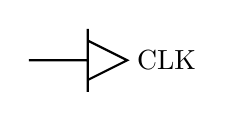
\begin{tikzpicture}
                \draw[thick] (-0.75, 0) -- (0,0)
                    (0,0.4) -- (0,-0.4)
                    (0,0.25) -- (0.5,0) -- (0,-0.25);
                \node[] at (1, 0) {CLK};
            \end{tikzpicture}
        \end{center}
        Input beim Übergang von \emph{$0 \rightarrow 1$} von CLK wirksam.
        \begin{center}
            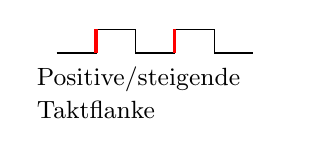
\begin{tikzpicture}
                \draw (0,0) -- (0.5, 0) -- (0.5, 0.3) -- (1, 0.3) -- (1, 0) -- (1.5, 0) -- (1.5, 0.3) -- (2, 0.3) -- (2, 0) -- (2.5, 0);
                \draw[very thick, red] (0.5, 0) -- (0.5, 0.3) (1.5, 0) -- (1.5, 0.3);
                \node[text width = 30mm] at (1.25, -0.5) {\small Positive/steigende Taktflanke};
            \end{tikzpicture}
        \end{center}
    \end{minipage}
    \hfill
    \begin{minipage}{0.45\linewidth}
        \begin{center}
            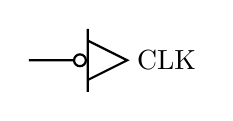
\begin{tikzpicture}
                \draw[thick] (-0.75, 0) -- (0,0)
                    (0,0.4) -- (0,-0.4)
                    (0,0.25) -- (0.5,0) -- (0,-0.25);
                \draw[thick, fill = white] (-0.1,0) circle [radius = 0.75mm];
                \node[] at (1, 0) {CLK};
            \end{tikzpicture}
        \end{center}
        Input beim Übergang von \emph{$1 \rightarrow 0$} von CLK wirksam.
        \begin{center}
            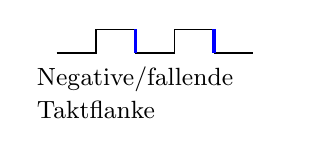
\begin{tikzpicture}
                \draw (0,0) -- (0.5, 0) -- (0.5, 0.3) -- (1, 0.3) -- (1, 0) -- (1.5, 0) -- (1.5, 0.3) -- (2, 0.3) -- (2, 0) -- (2.5, 0);
                \draw[very thick, blue] (1, 0.3) -- (1, 0) (2, 0.3) -- (2, 0);
                \node[text width = 30mm] at (1.25, -0.5) {\small Negative/fallende Taktflanke};
            \end{tikzpicture}
        \end{center}
    \end{minipage}
\end{center}
\subsubsection{D-FlipFlop}
\begin{center}
    \begin{minipage}[c]{0.35\linewidth}
        \begin{circuit}
            \node[dFf] (dff) {};
            
            \path[draw] (dff.pin 1) --++(180:0.4) node[fill=white] {\cirin{D}};
            \path[draw] (dff.pin 2) --++(180:0.4) node[fill=white] {\cirin{CLK}};
            \path[draw] (dff.pin 6) --++(0:0.4) node[fill=white] {\cirout{Q}};
            \path[draw] (dff.pin 4) --++(0:0.4) node[fill=white] {\ciroutn{Q}};
        \end{circuit}
    \end{minipage}
    \hfill
    \begin{minipage}[c]{0.6\linewidth}
        \begin{circuit}[0.35]
            \ctikzset{multipoles/flipflop/font = \footnotesize}
            \node[dLatch, flipflop def ={n2=1}, label={[font = \footnotesize, label distance = 5mm] 90:Master}] (dMaster) {};
            \node[dLatch, label={[font = \footnotesize, label distance = 5mm] 90:Slave}, right = of dMaster] (dSlave) {};

            \node[left = 4mm of dMaster.pin 1] (din) {\cirin{D}};
            \node[below = 5mm of din] (clk) {\cirin{CLK}};
            \node[right = 4mm of dSlave.pin 6] (q) {\cirout{Q}};
            \node[right = 4mm of dSlave.pin 4] (notq) {\ciroutn{Q}};
            
            \begin{pgfonlayer}{tl1}
                \node[circ, right = 1mm of clk] (nex1) {};
                \node[circ] at ($(dMaster.pin 6)!0.5!(dSlave.pin 1)$) (nex2) {};
            \end{pgfonlayer}

            \draw (din) -- (dMaster.pin 1);
            \draw (dMaster.pin 6) -- (nex2) -- (dSlave.pin 1);
            \draw (clk) -- (nex1) |- (dMaster-N2.west);
            \draw (nex1) --++ (0:1.2) |- (dSlave.pin 2);
            \path[draw] (nex2) --++(90:0.3) node[fill = white, font = \footnotesize] {X};
            \draw (dSlave.pin 6) -- (q);
            \draw (dSlave-N4.east) -- (notq);
        \end{circuit}
    \end{minipage}
\end{center}
\begin{equation*}
    Q_{n + 1} = \text{D} \quad \text{wenn} \quad \text{CLK}~0\rightarrow 1 
\end{equation*}
\begin{flushleft}
    \begin{tabular}{l l l}
        Master & low-active & $\text{CLK} = 0$\\
        Slave & high-active & $\text{CLK} = 1$\\
    \end{tabular}
\end{flushleft}
\subsubsection{SR-FlipFlop}
\begin{center}
    \begin{minipage}[c]{0.35\linewidth}
        \begin{circuit}
            \node[srFf] (srff) {};
            \path[draw] (dff.pin 1) --++(180:0.4) node[fill=white] {\cirin{D}};
            \path[draw] (dff.pin 2) --++(180:0.4) node[fill=white] {\cirin{CLK}};
            \path[draw] (dff.pin 3) --++(180:0.4) node[fill=white] {\cirin{R}};
            \path[draw] (dff.pin 6) --++(0:0.4) node[fill=white] {\cirout{Q}};
            \path[draw] (dff.pin 4) --++(0:0.4) node[fill=white] {\ciroutn{Q}};
        \end{circuit}
    \end{minipage}
    \hfill
    \begin{minipage}[c]{0.6\linewidth}
       \begin{circuit}[0.35]
        \ctikzset{multipoles/flipflop/font = \footnotesize}
        \node[srtLatch, flipflop def ={n2=1}, label={[font = \footnotesize, label distance = 5mm] 90:Master}] (srMaster) {};
        \node[srtLatch, label={[font = \footnotesize, label distance = 5mm] 90:Slave}, right = of dMaster] (srSlave) {};

        \node[left = 4mm of srMaster.pin 1] (sin) {\cirin{S}};
        \node[left = 4mm of srMaster.pin 3] (rin) {\cirin{R}};
        \node[below = 2mm of rin] (clk) {\cirin{CLK}};
        \node[right = 4mm of srSlave.pin 6] (q) {\cirout{Q}};
        \node[right = 4mm of srSlave.pin 4] (notq) {\ciroutn{Q}};

        \draw (sin) -- (srMaster.pin 1);
        \draw (rin) -- (srMaster.pin 3);
        \draw (srMaster.pin 6) -- (srSlave.pin 1);
        \draw (srMaster-N4.east) -- (srSlave.pin 3);
        \draw (srSlave.pin 6) -- (q);
        \draw (srSlave.pin 4) -- (notq);

        \begin{pgfonlayer}{tl1}
            \node[circ, right = 1mm of clk] (nex1) {}; 
        \end{pgfonlayer}
        \draw (clk) -- (nex1) |- (srMaster-N2.west);
        \draw (nex1) --++(0:1.2) |- (srSlave.pin 2);
       \end{circuit}
    \end{minipage}
\end{center}
\begin{equation*}
    Q_{n + 1} = \text{S} \lor \left(\overline{\text{R}} \land Q_n\right) \quad \text{wenn} \quad \text{CLK}~0\rightarrow 1 
\end{equation*}
\subsubsection{JK-FlipFlop}
\begin{center}
    \begin{minipage}[c]{0.33\linewidth}
        \begin{circuit}
            \node[jkFf] (jkff) {};
            \path[draw] (jkff.pin 1) --++(180:0.4) node[fill=white] {\cirin{J}};
            \path[draw] (jkff.pin 2) --++(180:0.4) node[fill=white] {\cirin{CLK}};
            \path[draw] (jkff.pin 3) --++(180:0.4) node[fill=white] {\cirin{K}};
            \path[draw] (jkff.pin 6) --++(0:0.4) node[fill=white] {\cirout{Q}};
            \path[draw] (jkff.pin 4) --++(0:0.4) node[fill=white] {\ciroutn{Q}};
        \end{circuit}
    \end{minipage}
    \hfill
    \begin{minipage}[c]{0.65\linewidth}
        \begin{circuit}
            \ctikzset{tripoles/european and port/height=0.3}
            \node[srFf] (srff) {};

            \node[and port, left = 3mm of srff.pin 1] (and1) {};
            \node[and port, left = 3mm of srff.pin 3] (and2) {};

            \node[left = 3mm of and1.in 2] (jin) {\cirin{J}};
            \node[left = 3mm of and2.in 1] (kin) {\cirin{K}};
            \node[left = 10mm of srff.pin 2] (clk) {\cirin{CLK}};           
            \node[right = 4.5mm of srff.pin 6] (q) {\cirout{Q} $= Q_1$};           
            \node[right = 4.5mm of srff.pin 4] (notq) {\ciroutn{Q} $= Q_2$};    
            
            \draw (and1.out) -- (srff.pin 1);
            \draw (and2.out) -- (srff.pin 3);
            \draw (jin) -- (and1.in 2);
            \draw (kin) -- (and2.in 1);
            \draw (clk) -- (srff.pin 2);

            \begin{pgfonlayer}{tl1}
                \node[circ, right = 0.8mm of srff.pin 6] (nex1) {};
                \node[circ, right = 2.4mm of srff.pin 4] (nex2) {};
            \end{pgfonlayer}
            \draw (srff.pin 6) -- (nex1) -- (q);
            \draw (srff.pin 4) -- (nex2) -- (notq);

            \draw (nex1) --++(270:1) -| (and2.in 2);
            \draw (nex2) --++(90:1) -| (and1.in 1);

            \node[label={[label distance = -1.5mm, font = \scriptsize] 90:$\text{S}_\text{i}$}] at ($(and1.out)!0.5!(srff.pin 1)$) {}; 
            \node[label={[label distance = -1.5mm, font = \scriptsize] 270:$\text{R}_\text{i}$}] at ($(and2.out)!0.5!(srff.pin 3)$) {}; 
        \end{circuit}
    \end{minipage}
\end{center}
\begin{equation*}
    Q_{n + 1} = \left(J \land \overline{Q_n}\right) \lor \left(\overline{K} \land Q_n\right) \quad \text{wenn} \quad \text{CLK}~0\rightarrow 1 
\end{equation*}
\begin{center}
    \begin{tabular}{c|c c|c c l}
        Fall & \textbf{J} & \textbf{K} & $Q_{1n + 1}$ & $Q_{2n + 1}$ & \\
        \cline{1-5}
        1 & $0$ & $0$ & $Q_{1n}$ & $Q_{2n}$ & speichern\\        
        2 & $0$ & $1$ & $0$ & $1$ & zurücksetzten\\        
        3 & $1$ & $0$ & $1$ & $0$ & setzen\\        
        4 & $1$ & $1$ & $\overline{Q_{1n}}$ & $\overline{Q_{2n}}$ & wechseln\\        
    \end{tabular}
\end{center}
Bei $\text{J}=\text{K}=1$ wechselt Output. (toggel)
\subsubsection{T-FlipFlop}
\begin{center}
    \begin{minipage}[t]{0.45\linewidth}
        \paragraph{V1} Ausgang wechselt bei jeder aktiven Taktflanke.
        \begin{circuit}
            \node[tFfv1] (tff) {};
            \path[draw] (tff.pin 2) --++(180:0.4) node[fill=white] {\cirin{CLK}};
            \path[draw] (tff.pin 6) --++(0:0.4) node[fill=white] {\cirout{Q}};
            \path[draw] (tff.pin 4) --++(0:0.4) node[fill=white] {\ciroutn{Q}};
        \end{circuit}
        \begin{align*}
            &Q_{n + 1} = \overline{Q_n}\\
            &\text{wenn CLK}~0\rightarrow 1 
        \end{align*}
    \end{minipage}
    \hfill
    \begin{minipage}[t]{0.45\linewidth}
        \paragraph{V2} Ausgang wechselt bei aktiver Taktflanke nur wenn \emph{$T = 1$}.
        \begin{circuit}[0.35]
            \node[tFfv2] (tff) {};
            \path[draw] (tff.pin 1) --++(180:0.4) node[fill=white] {\cirin{T}};
            \path[draw] (tff.pin 2) --++(180:0.4) node[fill=white] {\cirin{CLK}};
            \path[draw] (tff.pin 6) --++(0:0.4) node[fill=white] {\cirout{Q}};
            \path[draw] (tff.pin 4) --++(0:0.4) node[fill=white] {\ciroutn{Q}};
        \end{circuit}
        \begin{align*}
            &Q_{n + 1} = \overline{Q_n}\\
            &\text{wenn CLK}~0\rightarrow 1 \land T = 1
        \end{align*}
    \end{minipage}
\end{center}
\begin{center}
    \begin{minipage}[t]{0.3\linewidth}
        \begin{flushleft}
            BS V1
        \end{flushleft}
        \begin{circuit}[0.3]
            \ctikzset{multipoles/flipflop/font = \footnotesize}
            \node[dFf] (dff) {};

            \node[font = \small, left = 1mm of dff.pin 2] (clk) {\cirin{CLK}};
            \node[font = \small, right = 2.5mm of dff.pin 6] (q) {\cirout{Q}};
            \node[font = \small, right = 2.5mm of dff.pin 4] (notq) {\ciroutn{Q}};

            \begin{pgfonlayer}{tl1}
                \node[circ, right = 1mm of dff.pin 4] (nex1) {}; 
            \end{pgfonlayer}

            \draw (clk) -- (dff.pin 2);
            \draw (dff.pin 6) -- (q);
            \draw (dff-N4.east) -- (notq);
            \draw (nex1) --++(90:0.7) -| (dff.pin 1);
        \end{circuit}
    \end{minipage}
    \hfill\vline\hfill
    \begin{minipage}[t]{0.3\linewidth}
        \begin{flushleft}
            BS V1
        \end{flushleft}
        \begin{circuit}[0.3]
            \ctikzset{multipoles/flipflop/font = \footnotesize}
            \node[srFf] (srff) {};

            \node[font = \small, left = 1mm of srff.pin 2] (clk) {\cirin{CLK}};
            \node[font = \small, right = 2.5mm of srff.pin 6] (q) {\cirout{Q}};
            \node[font = \small, right = 2.5mm of srff.pin 4] (notq) {\ciroutn{Q}};

            \begin{pgfonlayer}{tl1}
                \node[circ, right = 0.7mm of srff.pin 4] (nex1) {}; 
                \node[circ, right = 1.4mm of srff.pin 6] (nex2) {}; 
            \end{pgfonlayer}

            \draw (clk) -- (srff.pin 2);
            \draw (srff.pin 6) -- (q);
            \draw (srff-N4.east) -- (notq);
            \draw (nex1) --++(90:0.7) -| (srff.pin 1);
            \draw (nex2) --++(270:0.7) -| (srff.pin 3);
        \end{circuit}
    \end{minipage}
    \hfill\vline\hfill
    \begin{minipage}[t]{0.3\linewidth}
        \begin{flushleft}
            BS V2
        \end{flushleft}
        \begin{circuit}[0.3]
            \ctikzset{multipoles/flipflop/font = \footnotesize}
            \node[jkFf] (jkff) {};

            \node[font = \small, left = 2.5mm of jkff.pin 1] (tin) {\cirin{T}};
            \node[font = \small, left = 2.5mm of jkff.pin 2] (clk) {\cirin{CLK}};
            \node[font = \small, right = 1mm of jkff.pin 6] (q) {\cirout{Q}};
            \node[font = \small, right = 1mm of jkff.pin 4] (notq) {\ciroutn{Q}};

            \begin{pgfonlayer}{tl1}
                \node[circ] at ($(tin)!0.7!(jkff.pin 1)$) (nex1) {}; 
            \end{pgfonlayer}

            \draw (tin) -- (jkff.pin 1);
            \draw (clk) -- (jkff.pin 2);
            \draw (jkff.pin 6) -- (q);
            \draw (jkff-N4.east) -- (notq);
            \draw (nex1) |- (jkff.pin 3);
        \end{circuit}
    \end{minipage}
\end{center}

\subsubsection{D-FlipFlop in CMOS-Technik}
\paragraph{Transmission Gates}
\begin{center}
    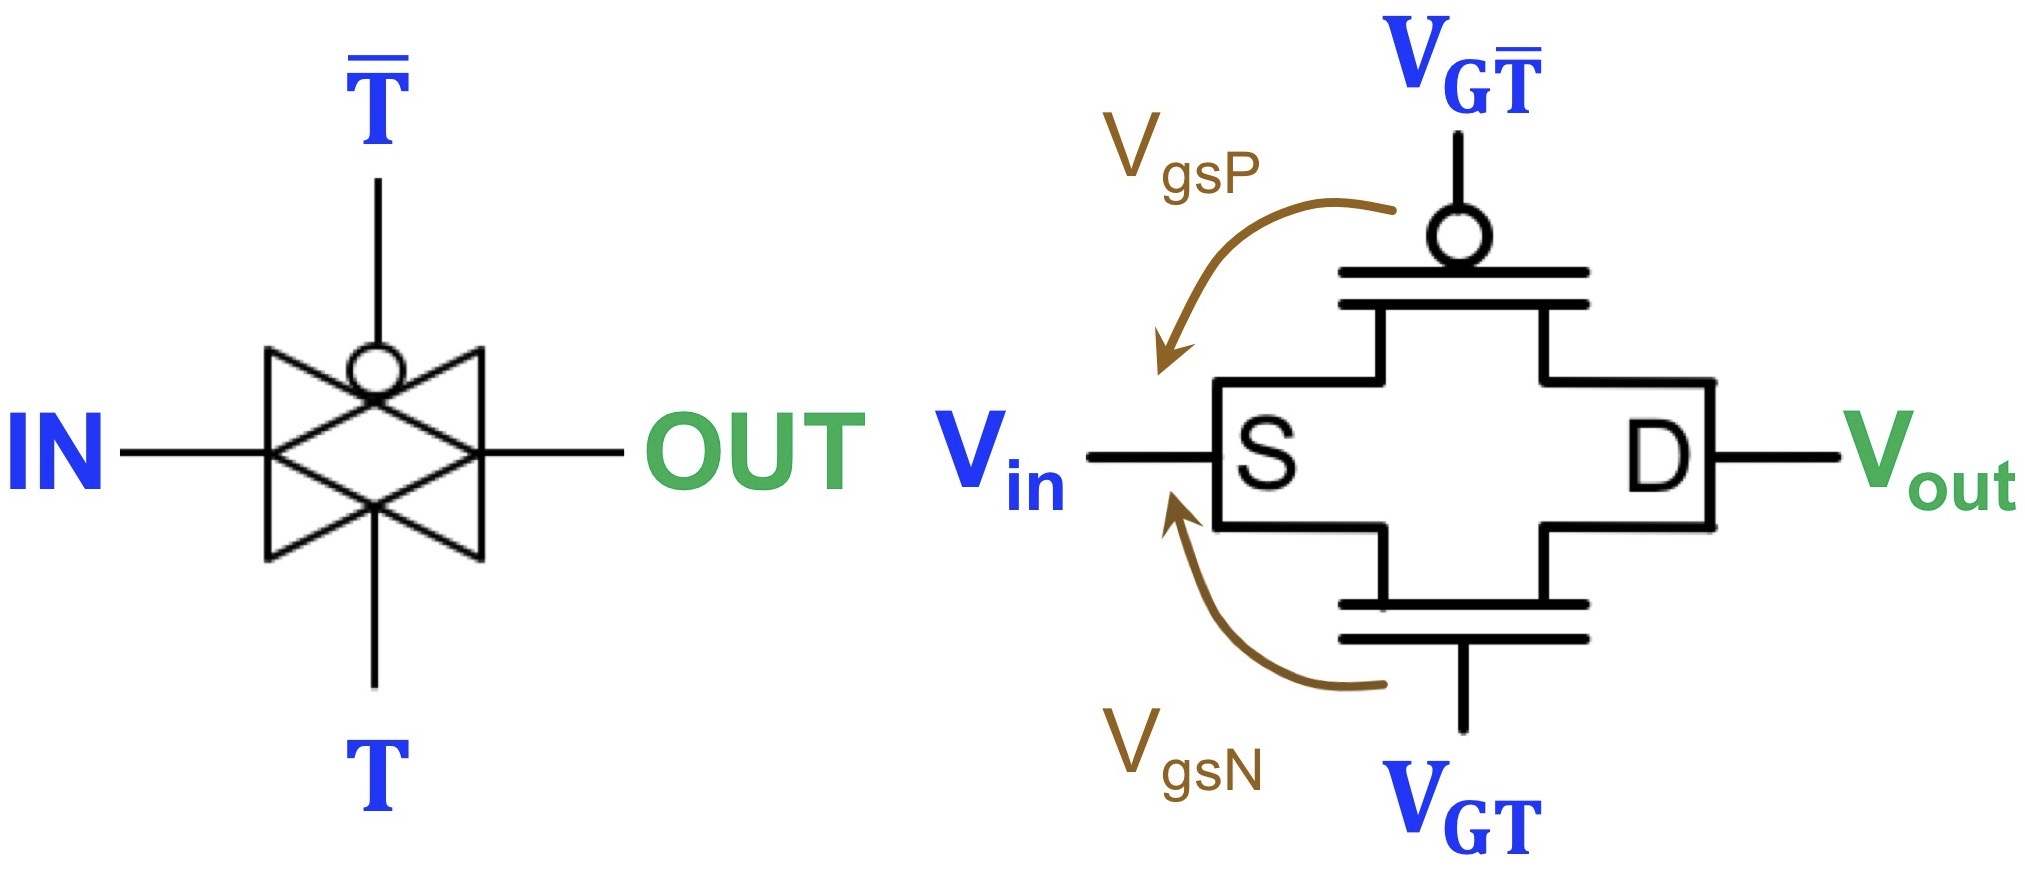
\includegraphics[height = 18mm]{images/tg.jpeg}
\end{center}
\begin{center}
    \small
    \begin{tabular}{c c|c|c}
        IN & T & Widerstand & OUT\\
        \hline
        0 & 0 & hochohm. & -\\
        0 & 1 & niederohm. & 0\\
        1 & 0 & hochohm. & -\\
        1 & 1 & niederohm. & 1\\
    \end{tabular}
\end{center}
TG sperrt wenn Widerstand hochohmig ist. ($\text{T}=0$)
\begin{center}
    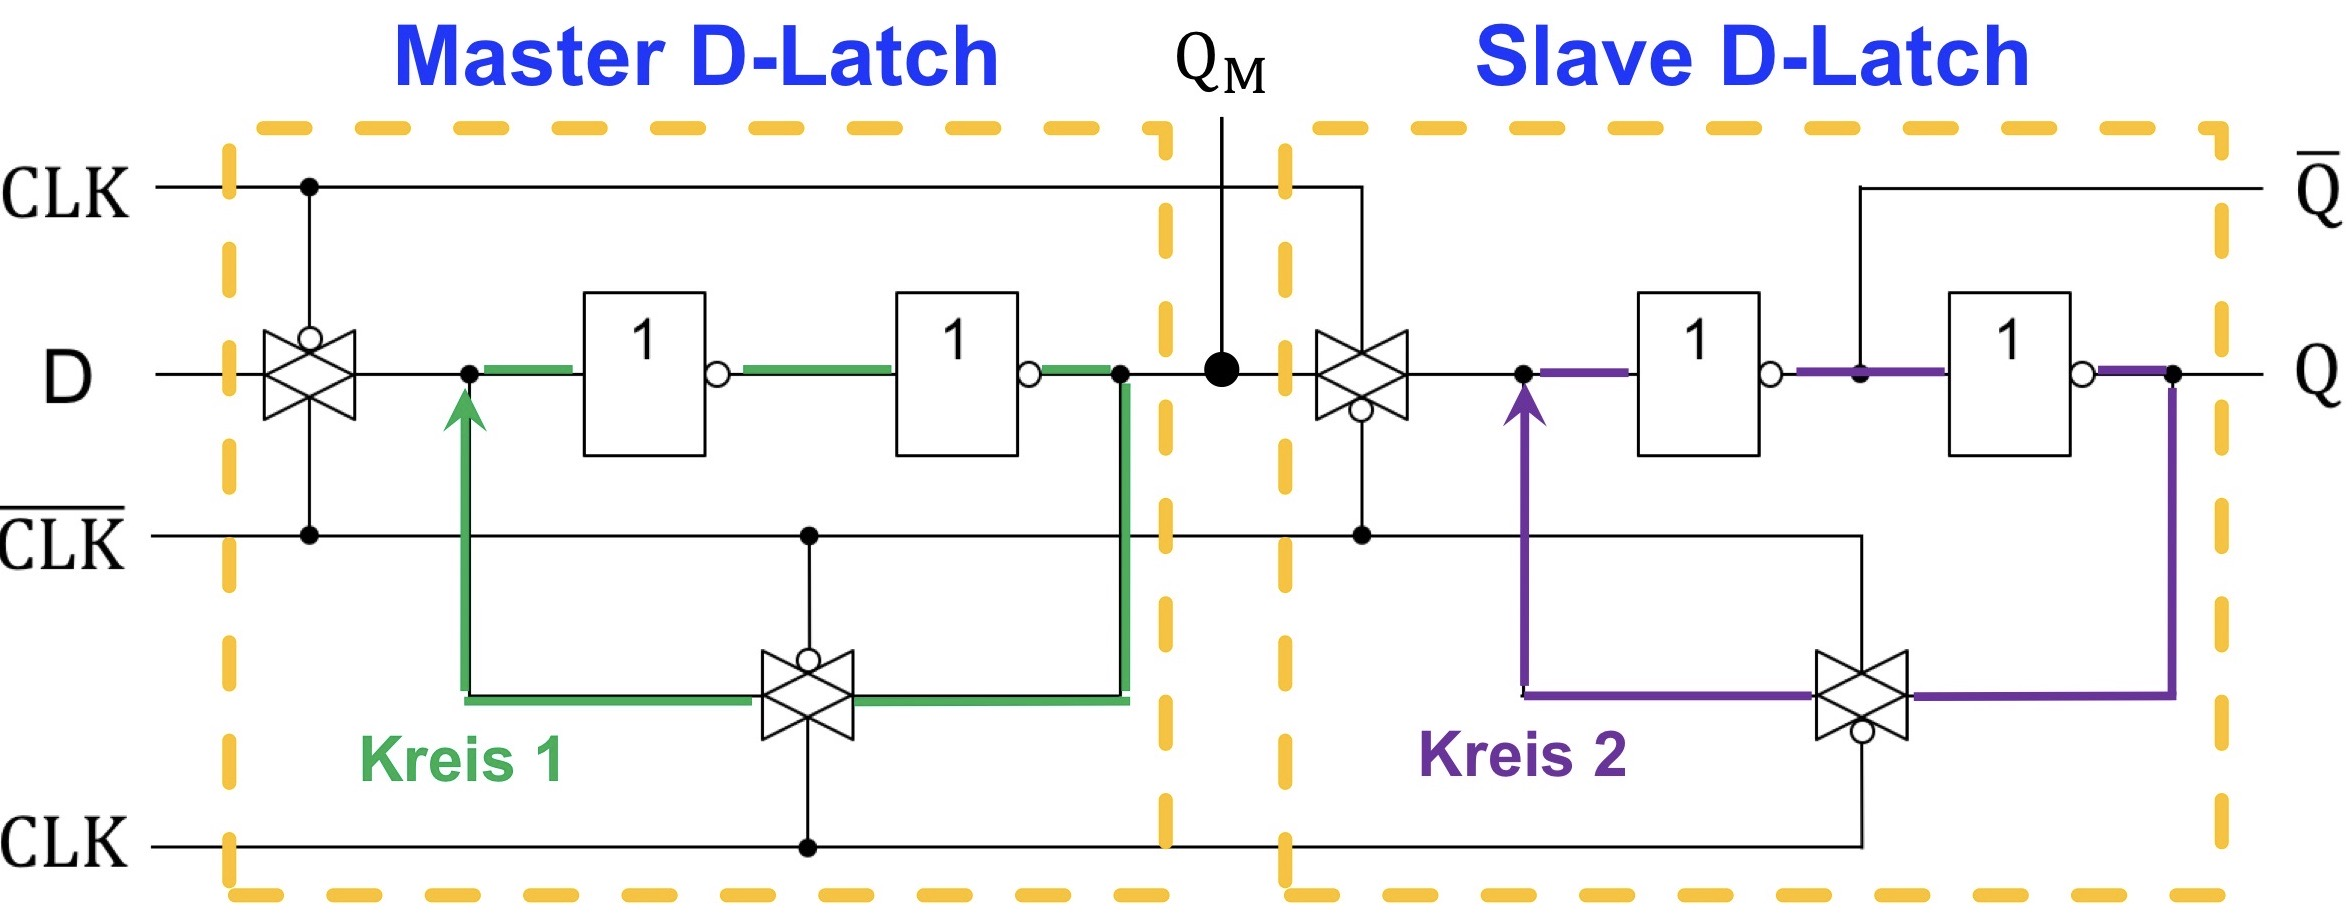
\includegraphics[width = 65mm]{images/d_ff_cmos.jpeg}
\end{center}
\begin{flushleft}
    \small
    \begin{tabular}{c l}
        CLK & \\
        0 & Input ins erste Latch übertragen\\
        1 & Latch verriegelt, Wert im Kreis gefangen
    \end{tabular}
\end{flushleft}
\begin{center}
    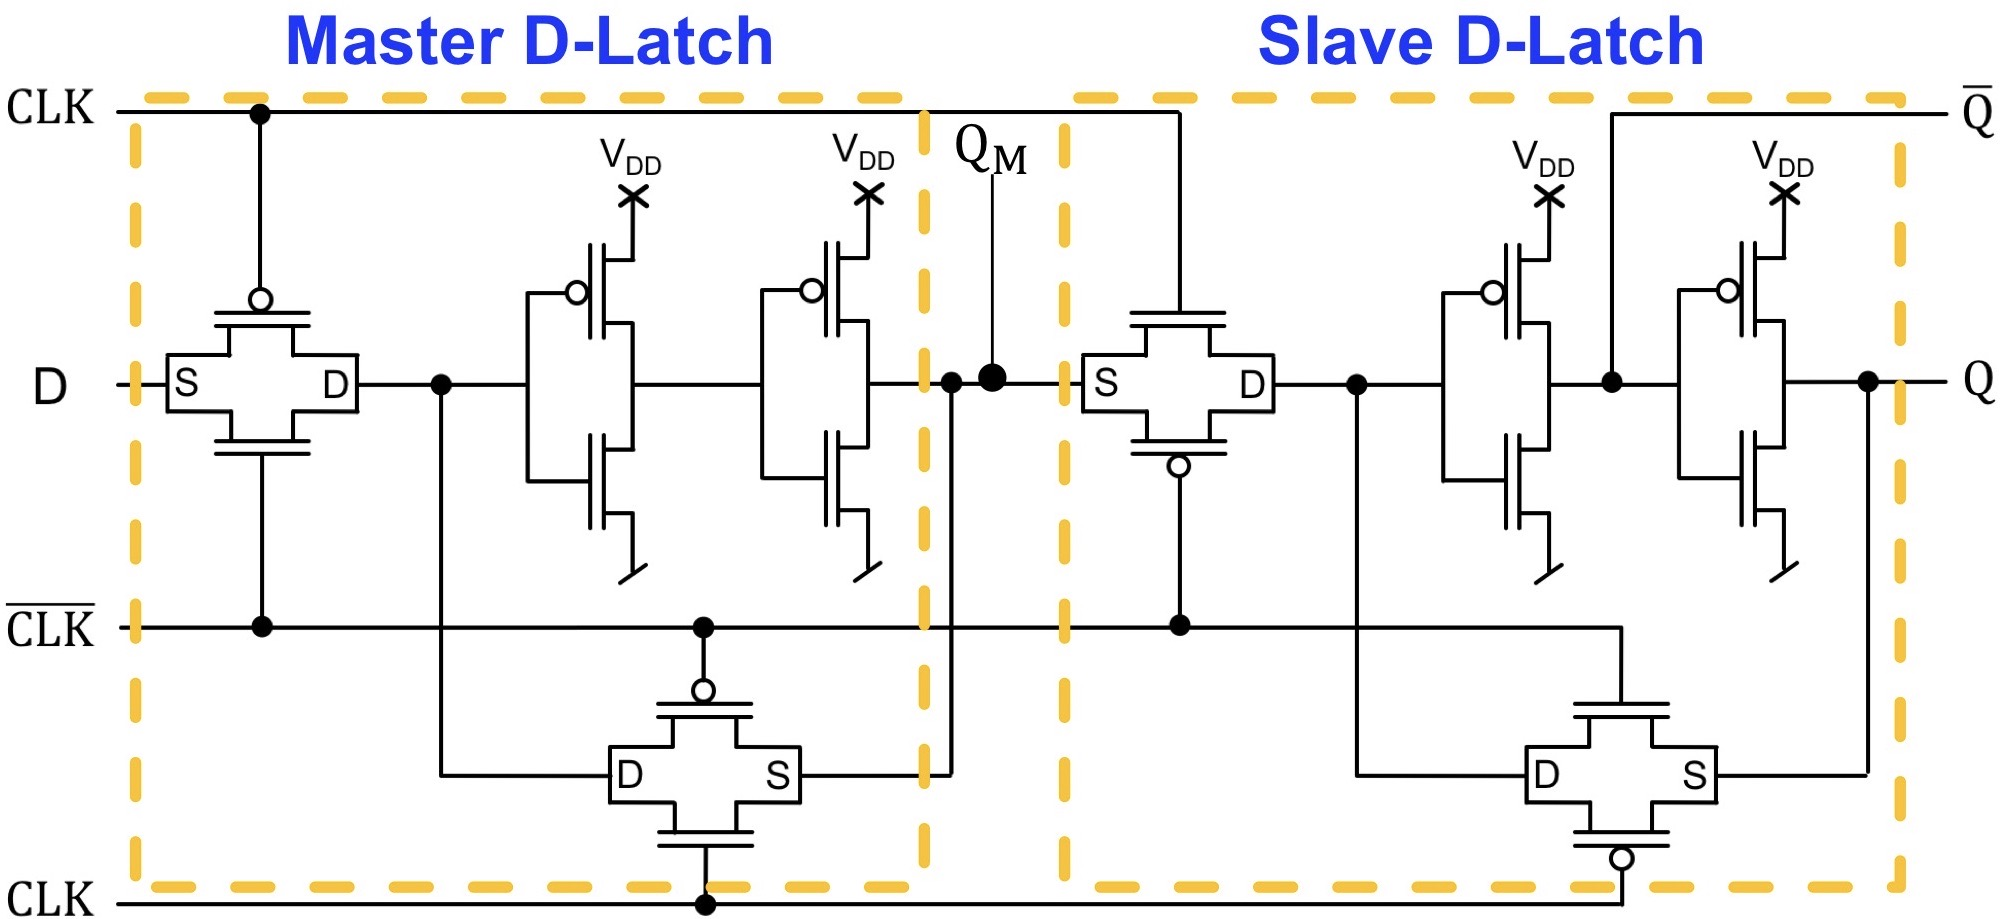
\includegraphics[width = 65mm]{images/d_ff_cmos_2.jpeg}
\end{center}
\subsubsection{D-FlipFlop $\Leftrightarrow$ JK-FlipFlop}
\begin{enumerate}
    \item JK-FF kann immer durch D-FF ersetzt werden.
    \begin{equation*}
        \text{D-FF:}\quad D_n = \left(J \land \overline{Q_n}\right) \lor \left(\overline{K} \land Q_n\right)\quad \text{:JK-FF}
    \end{equation*}
    \item Ein D-FF kann nur durch JK-FF ersetzt werden wenn:
    \begin{enumerate}
        \item Schaltung eine Rückkopplung enthält.
        \item Input D als $\left(F_1 \land \overline{Q_n}\right) \lor \left(F_2 \land Q_n\right)$ geschrieben werden kann.
    \end{enumerate}
\end{enumerate}
\paragraph{Gleichung für D-FF $\rightarrow$ JK-FF}
\begin{center}
    \begin{minipage}{0.65\linewidth}
        \begin{enumerate}
            \item Wahrheitstabelle mit Einängen und Rückkopplung.
            \item Wahrheitstabelle in \textcolor{pastelaqua}{$Q_n$} und \textcolor{pastelviolet}{$\overline{Q_n}$}.
            \item Separat Päckchen in \textcolor{pastelaqua}{$Q_n$} und \textcolor{pastelviolet}{$\overline{Q_n}$} machen.
            \item Päckchen mit OR verbinden. Ggf. \textcolor{pastelaqua}{$Q_n$} und \textcolor{pastelviolet}{$\overline{Q_n}$} ausklammern.
        \end{enumerate}
    \end{minipage}
    \hfill
    \begin{minipage}{0.3\linewidth}
        \begin{center}
            \begin{tikzpicture}
                \matrix (kv) [
                    matrix of nodes,
                    nodes in empty cells,
                    column sep=-\pgflinewidth, row sep=-\pgflinewidth,
                    nodes = {
                        rectangle,
                        draw = black,
                        text width = 1.3mm,
                        text height = 1.3mm,
                        align = center
                    }
                ]{
                \node[kvbinhead] {}; & \node[kvbinhead] {\tiny 00}; & \node[kvbinhead] {\tiny 01}; & \node[kvbinhead] {\tiny 11}; & \node[kvbinhead] {\tiny 10};\\
                \node[kvbinhead] {\tiny 00}; & & & &\\
                \node[kvbinhead] {\tiny 01}; & & & &\\
                \node[kvbinhead] {\tiny 11}; & & & &\\
                \node[kvbinhead] {\tiny 01}; & & & &\\
                };
    
                \node[] at ($(kv-1-1.north east) + (-1mm, -1mm)$) {\tiny $\text{Q}_\text{n}$A};
                \node[] at ($(kv-1-1.south west) + (1mm, 1mm)$) {\tiny BC};
                \draw[] ($(kv-1-1.north west) + (2mm, -2mm)$) -- (kv-1-1.south east);
                \fill[pastelviolet, opacity = 0.3] (kv-2-2.north west) rectangle (kv-5-3.south east);
                \fill[pastelaqua, opacity = 0.3] (kv-2-4.north west) rectangle (kv-5-5.south east);
            \end{tikzpicture}
        \end{center}
    \end{minipage}
\end{center}

\subsubsection{Asynchroner Set/Reset Input}
\begin{center}
    \begin{minipage}{0.45\linewidth}
        Können gespeicherte Zustände asynchron zu CLK überschreiben.
    \end{minipage}
    \hfill
    \begin{minipage}{0.5\linewidth}
        \begin{center}
            \begin{tikzpicture}
                \begin{pgfonlayer}{bg}
                    \node[draw, thick, minimum height = 10mm, minimum width = 7mm] at(0,0) (base) {};
                    \draw[thick] ($(base.170) +(0.01, 0)$) -- ($(base.180) + (0.1,0)$) -- ($(base.190) +(0.01, 0)$);
                    \node[point] (not) at ($(base.320) + (0.05,0)$) {};
                \end{pgfonlayer}
                \coordinate[label={[font = \footnotesize, label distance = 0mm]0:1D}] (d) at(base.140);  
                \coordinate[label={[font = \footnotesize, label distance = 0.5mm]0:C1}] (c) at(base.180);
                \coordinate[label={[font = \footnotesize, label distance = 0mm]90:R}] (r) at(base.250);  
                \coordinate[label={[font = \footnotesize, label distance = 0mm]90:S}] (s) at(base.290);  

                \path[draw] (d) --++(180:0.6) node[fill = white] {\cirin{D}};
                \path[draw] (c) --++(180:0.6) node[fill = white] {\cirin{CLK}};
                \path[draw] (base.40) --++(0:0.6) node[fill = white] {\cirout{Q}};
                \path[draw] (not) --++(0:0.55) node[fill = white] {\ciroutn{Q}};
                \path[draw] (r) --++(270:0.2) coordinate[pin={[pin distance = 2mm, font = \scriptsize, color = blue, text width = 12mm] 200:asynchroner Reset}] (rf);
                \path[draw] (s) --++(270:0.2) coordinate[pin={[pin distance = 1mm, font = \scriptsize, color = blue, text width = 12mm] 280:asynchroner Set}] (sf);
            \end{tikzpicture}
        \end{center}
    \end{minipage}
\end{center}

\subsubsection{Verzögerungszeiten}
\begin{flushleft}
    \small
    \begin{tabular}{l l p{32mm}}
        $t_s$ & Setup-Zeit & Solange muss Signal \underline{vor} aktiver Taktflanke stabil anliegen.\\
        $t_h$ & Hold-Zeit & Solange muss Signal \underline{nach} aktiver Taktflanke stabil anliegen.\\
        $t_{pd}$ & Verzögerungszeit & Durchlaufzeit
    \end{tabular}
\end{flushleft}
\begin{equation*}
    T_{\text{min}} \geq t_{\text{pd}1} + t_{\text{pd,ks}} + t_{\text{s}2} \qquad f_{\text{max}} = \frac{1}{T_{\text{min}}}
\end{equation*}
$t_h$ kann bei der Berechnung von $f_{\text{max}}$ vernachlässigt werden.\\
Es wird der längste PFad zwischen zwei FlipFlops betrachtet.

\subsubsection{Zwischenspeicher-FF}
\begin{center}
    \begin{minipage}[c]{0.35\linewidth}
        \begin{circuit}
            \node[jkFf, flipflop def ={t6={$\urcorner$}, t4={$\urcorner$}}] (jkff) {};
            \path[draw] (jkff.pin 1) --++(180:0.4) node[fill=white] {\cirin{J}};
            \path[draw] (jkff.pin 2) --++(180:0.4) node[fill=white] {\cirin{CLK}};
            \path[draw] (jkff.pin 3) --++(180:0.4) node[fill=white] {\cirin{K}};
            \path[draw] (jkff.pin 6) --++(0:0.4) node[fill=white] {\cirout{Q}};
            \path[draw] (jkff.pin 4) --++(0:0.4) node[fill=white] {\ciroutn{Q}};
        \end{circuit}
    \end{minipage}
    \hfill
    \begin{minipage}[c]{0.6\linewidth}
        \begin{circuit}
            \node[jkFf] (jkff1) {};
            \node[jkFf, right = of jkff1, flipflop def = {n2=1}] (jkff2) {};

            \path[draw] (jkff1.pin 1) --++(180:0.4) node[fill=white] {\cirin{J}};
            \path[draw] (jkff1.pin 2) --++(180:0.6) node[fill=white] {\cirin{CLK}};
            \path[draw] (jkff1.pin 3) --++(180:0.4) node[fill=white] {\cirin{K}};
            \path[draw] (jkff2.pin 6) --++(0:0.4) node[fill=white] {\cirout{Q}};
            \path[draw] (jkff2.pin 4) --++(0:0.4) node[fill=white] {\ciroutn{Q}};

            \begin{pgfonlayer}{tl1}
                \node[circ] at ($(clk)!0.8!(jkff1.pin 2)$) (nex1) {};
            \end{pgfonlayer}
            \draw (jkff1.pin 6) -- (jkff2.pin 1);
            \draw (jkff1.pin 4) -- (jkff2.pin 3);
            \draw (nex1) --++(270:0.7) --++ (0:1.6) |- (jkff2-N2.west);

            \node[label={[label distance = -1mm, font = \footnotesize] 90:$Q_i$}] at ($(jkff1.pin 6)!0.3!(jkff2.pin 1)$) {};
            \node[label={[label distance = -1mm, font = \footnotesize] 90:$\overline{Q_i}$}] at ($(jkff1.pin 4)!0.3!(jkff2.pin 3)$) {};
        \end{circuit}
    \end{minipage}
\end{center}
FlipFlop, dass Input bei steigender Taktflanke übernimmt und bei der nächsten fallenden Taktflanke ausgibt. (oder umgekehrte Flanken)
\begin{flushleft}
    \begin{tabular}{c l}
        $\urcorner$ & Ausgabe bei fallender Flanke\\
        $\lrcorner$ & Ausgabe bei steigender Flanke\\
    \end{tabular}
\end{flushleft}

\subsubsection{Frequenzteiler und Zähler}
\begin{center}
    \begin{minipage}{0.55\linewidth}
        \begin{circuit}[0.25]
            \ctikzset{multipoles/flipflop/clock wedge size=0.5}
            \node[tFfmin] (t1) {};
            \node[tFfmin, right = 6mm of t1] (t2) {};
            \node[tFfmin, right = 6mm of t2] (t3) {};
        
            \node[font = \footnotesize, left = 0.9mm of t1.pin 2] (clk) {\cirin{CLK}}; 
        
            \begin{pgfonlayer}{tl1}
                \node[circ] (nex1) at ($(t1.pin 6)!0.5!(t2.pin 1)$) {};
                \node[circ] (nex2) at ($(t2.pin 6)!0.5!(t3.pin 1)$) {};
            \end{pgfonlayer}
            \node[above = 4mm of nex1, font = \footnotesize] (lsb) {\cemph[secondaryheader]{LSB}};
            \node[above = 4.5mm of t3.pin 6, font = \footnotesize] (msb) {\cemph[secondaryheader]{MSB}};
        
            \draw (clk) -- (t1.pin 2);
            \draw (t1.pin 6) -- (nex1) |- (t2.pin 2);
            \draw (t2.pin 6) -- (nex2) |- (t3.pin 2);
            \path[draw] (nex1) -- (lsb) node[midway, left, font = \footnotesize] {$Q_1$}; 
            \path[draw] (nex2) --++ (90:0.45) node[midway, left, font = \footnotesize] {$Q_2$}; 
            \path[draw] (t3.pin 6) -- (msb) node[midway, right, font = \footnotesize] {$Q_3$}; 
        \end{circuit}
    \end{minipage}
    \hfill
    \begin{minipage}{0.4\linewidth}
        \begin{center}
            \begin{tikzpicture}
                \coordinate[label = {[font = \footnotesize]180:\cirin{CLK}}](clk) at (0,0.5);
                \coordinate[label = {[font = \footnotesize]180:$Q_1$}](q1) at (0,0);
                \coordinate[label = {[font = \footnotesize]180:$Q_2$}](q2) at (0,-0.5);

                \draw[thick] (clk) --++(0:0.4) --++(90:0.2) coordinate(f1t) --++(0:0.4) --++(270:0.2) --++(0:0.4) --++(90:0.2) coordinate(f2t) --++(0:0.4) --++(270:0.2) --++(0:0.4) --++(90:0.2)coordinate(f3t) --++(0:0.05);
                \draw[thick] (q1) --++(0:0.4) --++(90:0.2) --++(0:0.8) --++(270:0.2)coordinate(f2b) --++(0:0.8) --++(90:0.2) --++(0:0.05);
                \draw[thick] (q2) --++(0:0.4) coordinate(f1b) --++(90:0.2) --++(0:1.6) --++(270:0.2)coordinate(f3b) --++(0:0.05);

                \begin{pgfonlayer}{tl1}
                    \draw[thick, dashed, red] (f1t) -- (f1b);
                    \draw[thick, dashed, red] (f2t) -- (f2b);
                    \draw[thick, dashed, red] (f3t) -- (f3b);
                \end{pgfonlayer}
            \end{tikzpicture}
        \end{center}
    \end{minipage}
\end{center}
Kaskadieren von T-Flipflops führt zu einer Frequenzreduktion von CLK um Faktor 2.\\
Kann als Bitzähler verwendet werden (ohne CLK). MSB ist längste Frequenz. $n_{T,ff} \rightarrow 0\dots (2^n -1)$